\documentclass[12pt]{extarticle}
\usepackage[utf8]{inputenc}
\usepackage{graphicx}
\usepackage{float}

% Disable indentation
\setlength{\parindent}{0pt}

\title{Lab 7: Network virtualization with Virtualbox}
\author{Alexander Hoffmann}
\date{\today}

\begin{document}

\maketitle

\section{NAT mode}
\textbf{1.} The IP configuration of the host machine can be determined using \texttt{ifconfig}.\\~\\
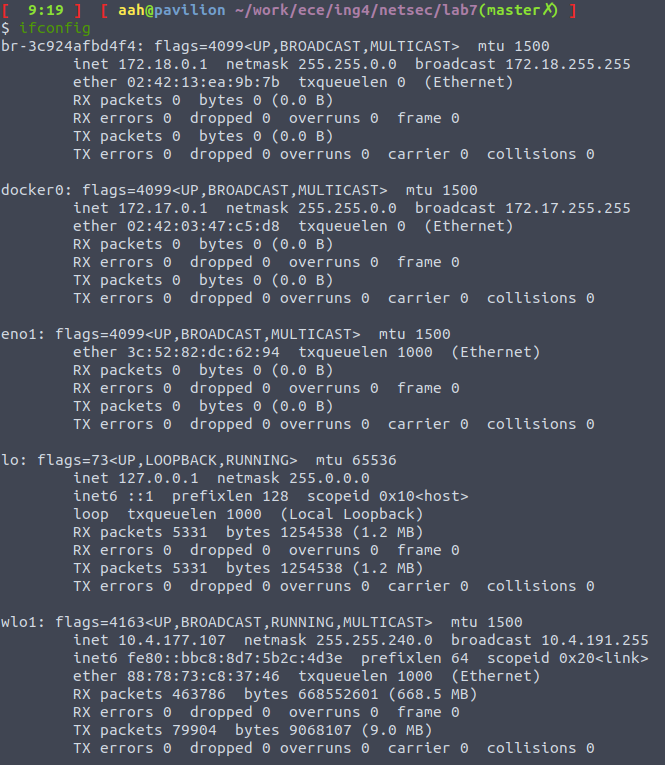
\includegraphics[scale=0.6]{resources/1-1.png}\\

\textbf{2.} We use the same command in the virtual machine.\\~\\
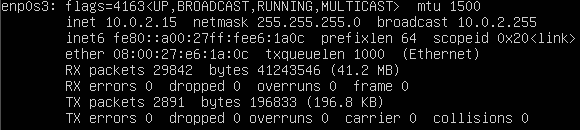
\includegraphics[scale=0.7]{resources/1-2.png}\\

\textbf{3.} It seems like the host machine and the virtual machine are not on the same network. This is because the VM is connected through NAT.\\

\textbf{4.} To get the DHCP server address, we use the following command:
\begin{verbatim}
sudo grep -R "DHCPOFFER" /var/log/*
\end{verbatim}
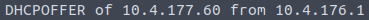
\includegraphics[scale=0.7]{resources/1-4.png}\\
This corresponds to the DHCP server address on the host machine. Now let's see which IP the DHCP server has on the VM.\\~\\
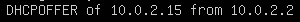
\includegraphics[scale=0.8]{resources/1-4-2.png}\\

\textbf{5.} The IP address of the NAT device is 10.0.2.15.

\textbf{6.} Since the VM is a server, it does not have a virtual interface. Therefore, we will be using \texttt{tcpdump} to capture traffic. More specifically, to filter the DHCP protocol, we use the following:
\begin{verbatim}
tcpdump -i eth0 -pvn port 67 and port 68
\end{verbatim}
Now we have to renew the DHCP lease. To do this, use:
\begin{verbatim}
dhclient enp0s3
\end{verbatim}
Which will display the following packets.\\~\\
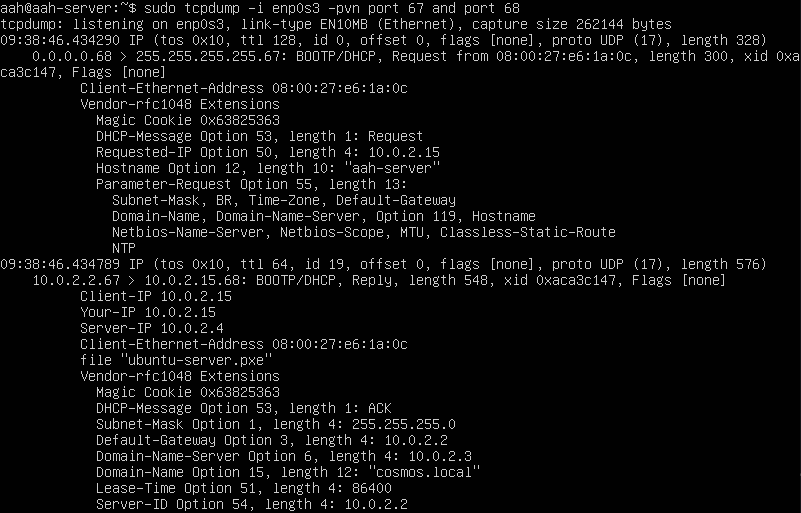
\includegraphics[scale=0.5]{resources/1-5.png}\\
We can observe that the VM broadcasts a DHCP Request. The DHCP server then sends a DHCP Reply with a lease.

\textbf{7.} There is no direct traffic between the DHCP server and the VM. In fact, the host machine is the DHCP server for the VM. This is why we are not capturing any traffic going to the VM.\\~\\
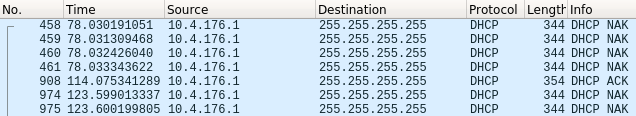
\includegraphics[scale=0.6]{resources/1-7.png}\\

\textbf{8.} Once again, since the VM does not have a graphical interface, we will use the \texttt{ping} command to observe the traffic. Suppose we ping google.com from the VM. Here is the traffic captured by Wireshark on the host machine.\\~\\
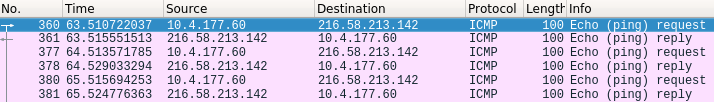
\includegraphics[scale=0.6]{resources/1-8.png}\\
Now let's observe the ping from the host.\\~\\
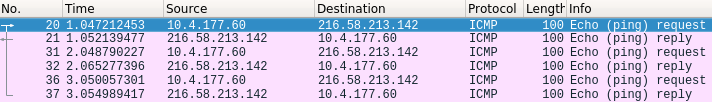
\includegraphics[scale=0.6]{resources/1-8-1.png}\\
The packets are simingly the same except that the header is slightly different.\\

\section{Host-only mode}
\textbf{9.} The IP address of the host has not changed. See question 1.\\ 

\textbf{10.} Now let's take a look at the IP configuration of the VM.\\~\\
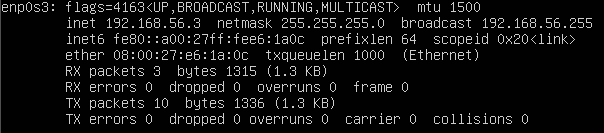
\includegraphics[scale=0.7]{resources/2-9.png}\\
The IP address of the network is 192.168.56.1/24. It is a private network linked to a virtual interface created by VirtualBox.\\

\textbf{11.} To find out the IP address of the DHCP server, we use the same command as before. This time, the DHCP server is 192.168.56.2. Note that the IP address of the interface on the host machine is 192.168.56.1.\\~\\
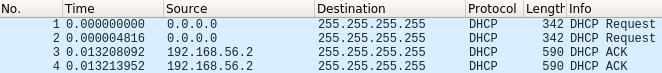
\includegraphics[scale=0.6]{resources/q11.png}\\

\section{Bridged mode}
\textbf{13.} For this section, we have changed location. Therefore, the IP address is not the same as previously.\\~\\
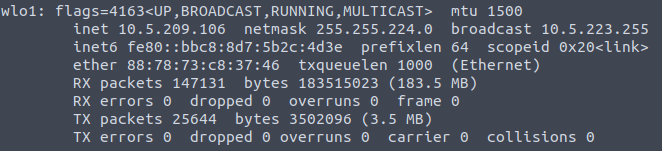
\includegraphics[scale=0.6]{resources/13.png}\\

\textbf{14.} Now that we are in bridged mode, the VM is directly connected to the same network as the host.\\~\\
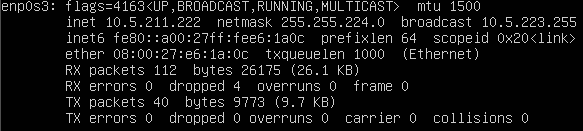
\includegraphics[scale=0.7]{resources/14.png}\\

\textbf{15.} Bridged mode replicates another node on the physical network and the VM will receive it's own IP address if DHCP is enabled in the network. It can be accessed by all computers in your host network.\\

\textbf{16.} To find the DHCP, use:
\begin{verbatim}
sudo grep -R "DHCPOFFER" /var/log/syslog
\end{verbatim}
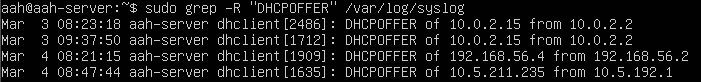
\includegraphics[scale=0.6]{resources/15.png}\\
The last line corresponds to the DHCP offer from the server. The IP address of the server is 10.5.192.1.\\

\textbf{17.} To request a new lease from the DHCP server, we use:
\begin{verbatim}
sudo dhclient <interface>
\end{verbatim}
If we apply it to the VM, here is the traffic captured by wireshark:\\~\\
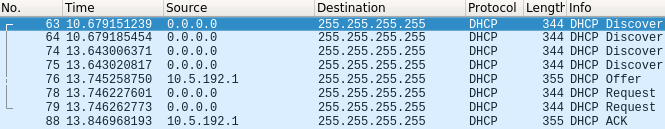
\includegraphics[scale=0.6]{resources/16.png}\\
In this case, we requested a new lease and the DHCP responded with the same IP address. Suppose we would leave and come back the next day, the DHCP would send us another IP address because the one we currently have might already have been taken by another device on the network.\\

\textbf{18.} 
Typically, when a router goes to establish an IP address for a client computer it is given the initial IP address of 255.255.255.255 or "static." With DHCP, that initial IP address is assigned to a computer that is now configured to use that IP address as its primary address.

Using a DHCP server allows you to specify how to address your network in the future. If the DHCP server isn't configured to allocate any addresses to your network, the computer will ask the DHCP server for a new address periodically. In the future, whenever your network changes and you switch over to using DHCP, it will automatically get assigned a new IP address.\\

\textbf{19.} The same applies for the virtual machine. In bridge mode, both the host machine and the VM are individual devices since virtualbox simulates a network interface for the VM.\\~\\
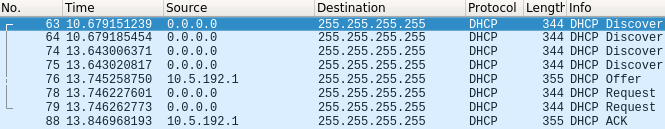
\includegraphics[scale=0.6]{resources/16.png}\\

\textbf{20.} A DHCP lease is a temporary assignment of an IP address to a device on the network. When using DHCP to manage a pool of IP addresses, each client served on the network is only “renting” its IP address. Thus, IP addresses managed by a DHCP server are only assigned for a limited period of time. When there is no more use for an IP address, it is released from the DHCP lease and may be assigned by another DHCP server without causing any further problems.

\end{document}
